\documentclass[11pt,a4paper]{article}

% ---------- packages ----------
\usepackage[T1]{fontenc}
\usepackage[utf8]{inputenc}
\usepackage[a4paper,margin=2.4cm]{geometry}
\usepackage[protrusion=true,expansion=false]{microtype}
\usepackage{amsmath,amssymb}
\usepackage{booktabs}
\usepackage{array}
\usepackage{tabularx}
\usepackage{xcolor}
\usepackage{enumitem}
\usepackage{listings}
\usepackage{tikz}
\usetikzlibrary{positioning,arrows.meta,shapes.geometric,fit,backgrounds,calc}
\usepackage[hidelinks]{hyperref}

% ---------- listings style ----------
\definecolor{cfgray}{gray}{0.45}
\lstdefinestyle{cf}{
  basicstyle=\ttfamily\footnotesize,
  breaklines=true,
  breakatwhitespace=false,
  columns=fullflexible,
  keepspaces=true,
  showstringspaces=false,
  frame=single,
  rulecolor=\color{cfgray!60},
  backgroundcolor=\color{gray!4},
  numbers=none,
  xleftmargin=6pt,
  framexleftmargin=6pt,
  aboveskip=8pt,
  belowskip=8pt,
}
\lstset{style=cf}

% ---------- tabularx helpers ----------
\newcolumntype{L}{>{\raggedright\arraybackslash}X}
\renewcommand{\arraystretch}{1.25}

% ---------- inline label helpers for assumptions / invariants ----------
\newcommand{\Aref}[1]{\textbf{A#1}}
\newcommand{\Iref}[1]{\textbf{I#1}}

% ---------- title ----------
\title{\vspace{-1.0cm}\textbf{A SWIFT-Native Control Function}\\[2pt]
\large Specialising an asset-agnostic compliance, freeze and validation control
to Swift's shared ledger, identity and compliance estate\\[2pt]
\normalsize\itshape with an explicit trust model, epoch-bound freshness,
composable per-asset policy, and verifiable cross-ledger enforcement}

\begin{document}
\maketitle

\begin{abstract}
\noindent
A companion design specifies an \emph{asset-agnostic} smart-contract control
function: one decision component, exposed through a stable interface, bound to
each ledger by a thin adapter, and aligned with ISO~20022 and the FATF~R.16 /
IVMS101 Travel-Rule model. That design is deliberately portable. This document
\emph{specialises} it to the infrastructure Swift is actually building, so that
the control function is not merely \emph{compatible} with Swift but \emph{native}
to it --- and it does so under the discipline an interoperability protocol team
would demand: a stated trust model, security properties that hold \emph{under
named assumptions}, and verifiable rather than asserted guarantees. Swift's
shared ledger MVP is an EVM-compatible chain on Hyperledger Besu that Swift
operates while banks retain keys and assets; Swift is the certification authority
behind its PKI and the 3SKey key-share solution; the KYC Registry, Transaction
Screening and Sanctions List Monitor are live compliance services keyed on the
BIC; and MyStandards with the SMPG/CBPR+ machinery governs message
specifications. We map the Policy
Enforcement/Decision/Information/Administration (PEP/PDP/PIP/PAP) reference model
onto these components, then strengthen the design in six ways. (1) We state an
explicit \textbf{trust model} --- six assumptions, seven adversaries and nine
invariants --- so each property is conditional and falsifiable. (2) We replace wall-clock
attestation expiry with \textbf{epoch-bound freshness}: a single on-chain epoch
bump invalidates every stale ``clear'' at once, turning the largest residual risk
into a one-write safety invariant. (3) We make asset-agnosticism
\emph{structural} via a \textbf{per-asset policy registry} of composable rule
modules behind a fixed engine. (4) Every decision commits an \textbf{evidence
hash} binding it to the exact inputs screened, making it non-repudiable and
auditable. (5) We govern the signer through an on-chain \textbf{signer-key
registry} with rotation and break-glass, rather than a static pin. (6) Cross-ledger
projection is upgraded from ``identical by conformance'' to ``verified by
\textbf{enforcement receipt}'', mirroring the commit/execute separation and
independent risk layer of mature cross-chain protocols; we also fix a latent
correctness gap in quantity-bounded rules across ledgers. The one genuinely new
primitive remains a signed \emph{wallet-to-BIC} binding, now given an explicit
\textbf{revocation lifecycle}: a sticky, governed binding revocation that a
re-screen cannot undo (invariant \Iref{9}). Three further refinements close the
gaps a protocol review would flag: that binding revocation; \textbf{operator
sequencing accountability}, argued from Besu's QBFT validator set rather than
assumed; and an explicit \textbf{transaction-graph confidentiality} posture for a
permissioned ledger. We close with a progressive trust-minimisation roadmap and
are explicit about what Swift's estate does \emph{not} give us --- investor-level
KYC, a productised signer, custody --- so the proposal is buildable rather than
aspirational.
\end{abstract}

\newpage
\tableofcontents
\vspace{0.5cm}
\newpage

% =====================================================================
\section{From asset-agnostic to Swift-native}
\label{sec:intro}

\subsection{What changes, and why now}
The companion design argues that control logic (who may do what, under which
conditions, and what is emitted) should be defined independently of token
mechanics, so that one control function serves any asset on any ledger behind a
thin per-platform adapter. That portability is the right \emph{property}, and we
keep it. What has changed is that Swift is no longer an abstract ``neutral
orchestrator'' to design \emph{towards}: it is a concrete stack to build
\emph{on}. In September~2025 Swift announced a blockchain-based shared ledger; by
January~2026 it had completed a delivery-versus-payment trial of tokenised bonds
with BNP~Paribas Securities Services, Intesa~Sanpaolo and
Soci\'et\'e~G\'en\'erale--FORGE; and by March~2026 it had finished the design
phase and begun building the MVP, targeting live transactions within the
year~\cite{swiftledgerpr,swiftmvp,fstrial}.

Three facts about that stack drive every design choice below:
\begin{enumerate}[leftmargin=1.5em,itemsep=2pt]
  \item \textbf{The home ledger is EVM.} The MVP is built on Hyperledger Besu
  with an EVM-compatible architecture~\cite{swiftmvp}. The Solidity
  \texttt{IControlFunction} therefore deploys \emph{natively} on Swift's own
  chain --- no adapter is needed for the home case; adapters are reserved for
  \emph{external} ledgers reached through Swift's orchestration. Besu's
  permissioned BFT consensus (QBFT/IBFT) gives \emph{deterministic finality},
  which we rely on explicitly in assumption~\Aref{1}.
  \item \textbf{Swift operates, banks custody.} Swift provides ``orchestration of
  transaction workflows, validation of funding commitments and coordination of
  interbank processes,'' while banks ``retain full authority over keys, assets,
  funding and settlement''~\cite{swiftmvp}. This is a PEP/PDP \emph{coordination}
  role, and it draws a hard line: \textbf{the function decides and emits; it
  never custodies or moves value.}
  \item \textbf{The trust root already exists.} Swift is the certification
  authority for its PKI and for 3SKey, whose ``Digital'' variant uses a
  device-bound key-share model~\cite{swift3skey,swiftpki,swift3skeyfs}. The
  off-chain signer is not a new trust anchor to bootstrap; it is a module that
  chains to a CA institutions already trust.
\end{enumerate}

\subsection{Design thesis, restated for Swift}
\textbf{The control function is a Swift-operated decision and event component
that lives natively on the Besu shared ledger, draws its attributes from Swift's
existing compliance and identity services, signs off-chain decisions with a
threshold module rooted in Swift's CA, and projects the same decision onto
external ledgers through Swift's orchestration connector under a verified
enforcement contract.} Asset-agnosticism is preserved --- the decision logic
operates on an abstract request behind a fixed engine --- but the
\emph{deployment} is opinionated: one home ledger, many reachable ledgers, one
compliance estate behind all of them, and one explicit trust model
(Section~\ref{sec:trust}) that every later claim refers back to.

% =====================================================================
\section{The Swift stack we build on}
\label{sec:stack}

Before mapping the reference model we fix exactly which Swift components are real
today and what each provides. Nothing below is hypothetical; the only new
artefact this design introduces is the wallet-to-BIC binding of
Section~\ref{sec:identity}. Two design-relevant properties we additionally
require of the PIPs --- a monotonic \emph{epoch} on each sanctions-list
publication and a per-record \emph{version} on registry changes --- are exposed
today as change notifications and audit metadata; we use them in
Section~\ref{sec:freshness}.

\begin{table}[h]
\centering
\caption{Concrete Swift components and the role each plays in the control
function. ``New'' marks the single primitive that does not exist today.}
\label{tab:stack}
\begin{tabularx}{\textwidth}{@{}p{3.5cm} L p{3.0cm}@{}}
\toprule
\textbf{Swift component} & \textbf{What it is today} & \textbf{Role here} \\
\midrule
Shared ledger (MVP) & EVM-compatible permissioned chain on Hyperledger Besu;
Swift orchestrates, banks hold keys/assets~\cite{swiftmvp}. & Home PEP + on-chain
fast-path PDP. \\
Orchestration / connector & Coordinates interbank workflow, validates funding
commitments; prior trials used a Swift connector and Chainlink CCIP/CRE to reach
external chains~\cite{swiftmvp,swiftchainlink23,swiftcbdc}. & Cross-ledger
projection; commit/execute coordination. \\
KYC Registry & BIC-keyed institutional due-diligence utility, 7{,}700+
institutions; owner controls access with full audit trail; API channel for
real-time change monitoring; ISSA DDQ securities module~\cite{swiftkyc,swiftkycdata}. &
Institutional eligibility PIP; registry-epoch source. \\
Transaction Screening & Fully managed real-time sanctions screening; Smart
Screening uses ISO~20022 data to cut false positives~\cite{swifttxnscreen}. &
Sanctions/AML PIP (off-chain rule). \\
Sanctions List Monitor & Instant alerts on sanctions-list changes, standardised
format~\cite{swiftslm}. & List-epoch advance trigger. \\
PKI / 3SKey & Swift is the CA; FIPS~140-2 HSM tokens; 3SKey Digital uses
device-bound key shares~\cite{swift3skey,swiftpki,swift3skeyfs}. & Trust root for
the threshold signer; signer-registry anchor. \\
MyStandards + SMPG/CBPR+ & Web platform where 150+ orgs publish ISO~20022 usage
guidelines, with a Readiness Portal for testing; market-practice governance via
SMPG/PMPG~\cite{swiftmystd,swiftsmpg}. & Conformance + certification vectors +
governance channel. \\
\bottomrule
\end{tabularx}
\end{table}

% =====================================================================
\section{Mapping the reference model onto Swift}
\label{sec:arch}

The companion design structures the function as PEP (enforcement), PDP
(decision), PIP (information) and PAP (administration). Each plane now has a named
Swift home (Figure~\ref{fig:arch}).

\begin{figure}[h]
\centering
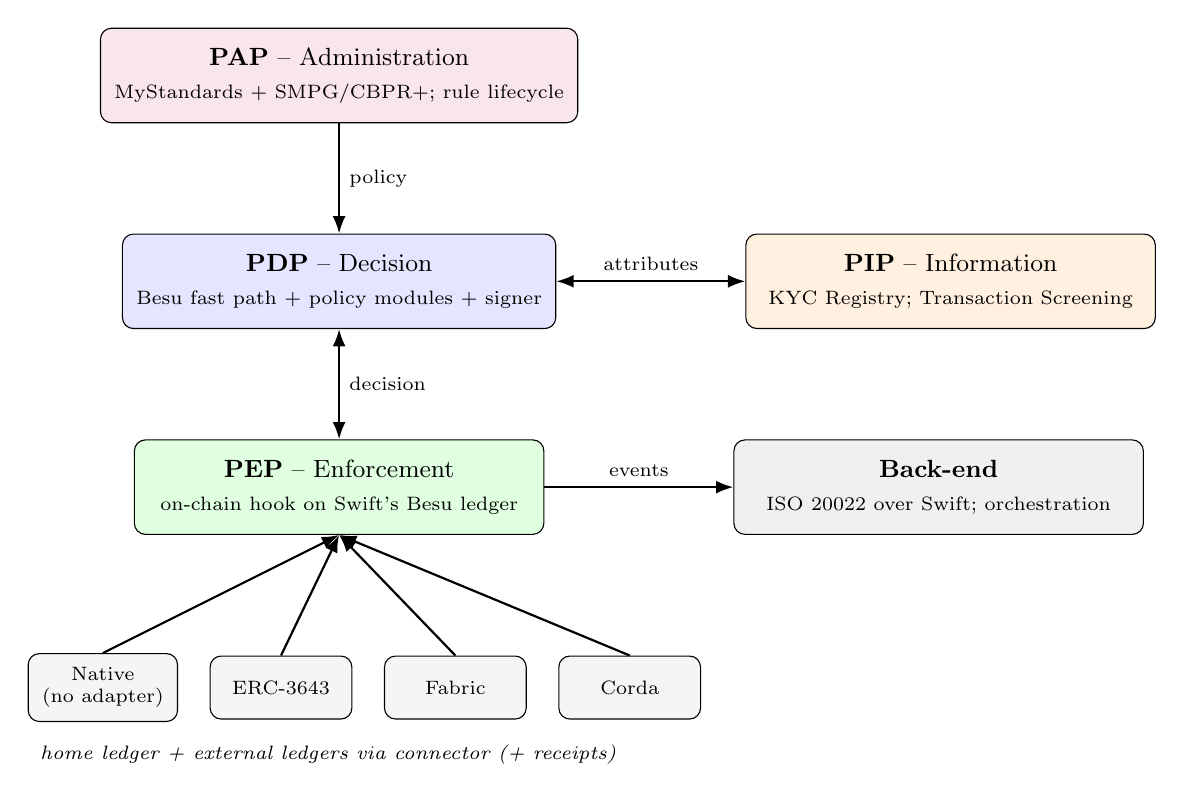
\begin{tikzpicture}[
  box/.style={draw, rounded corners, align=center, inner sep=5pt, font=\small},
  plane/.style={box, minimum width=52mm, minimum height=12mm},
  small/.style={box, fill=gray!8, font=\scriptsize, minimum height=8mm, minimum width=18mm},
  arr/.style={-{Latex[length=2.2mm]}, thick},
  darr/.style={{Latex[length=2.2mm]}-{Latex[length=2.2mm]}, thick},
]
\node[plane, fill=purple!10] (pap) {\textbf{PAP} -- Administration\\[1pt]\scriptsize MyStandards + SMPG/CBPR+; rule lifecycle};
\node[plane, fill=blue!10, below=14mm of pap] (pdp) {\textbf{PDP} -- Decision\\[1pt]\scriptsize Besu fast path + policy modules + signer};
\node[plane, fill=orange!12, right=24mm of pdp] (pip) {\textbf{PIP} -- Information\\[1pt]\scriptsize KYC Registry; Transaction Screening};
\node[plane, fill=green!12, below=14mm of pdp] (pep) {\textbf{PEP} -- Enforcement\\[1pt]\scriptsize on-chain hook on Swift's Besu ledger};
\node[plane, fill=gray!12, right=24mm of pep] (iso) {\textbf{Back-end}\\[1pt]\scriptsize ISO 20022 over Swift; orchestration};

\node[small, below=15mm of pep, xshift=-30mm] (a0) {Native\\(no adapter)};
\node[small, right=4mm of a0] (a2) {ERC-3643};
\node[small, right=4mm of a2] (a4) {Fabric};
\node[small, right=4mm of a4] (a5) {Corda};
\node[below=2mm of a2, font=\scriptsize\itshape, xshift=6mm] (alab) {home ledger + external ledgers via connector (+ receipts)};

\draw[arr] (pap) -- node[right,font=\scriptsize]{policy} (pdp);
\draw[darr] (pdp) -- node[right,font=\scriptsize]{decision} (pep);
\draw[darr] (pdp) -- node[above,font=\scriptsize]{attributes} (pip);
\draw[arr] (pep) -- node[above,font=\scriptsize]{events} (iso);
\draw[arr] (a0.north) -- (pep.south);
\foreach \a in {a2,a4,a5} {\draw[arr] (\a.north) -- (pep.south);}
\end{tikzpicture}
\caption{The reference model, specialised. The home ledger needs no adapter
because it is itself EVM; external ledgers attach through Swift's orchestration
connector and return enforcement receipts. The PIP and signer are existing Swift
services rather than bespoke oracles.}
\label{fig:arch}
\end{figure}

\paragraph{PEP --- enforcement on the Besu ledger.} On the home ledger the
enforcement hook is an ordinary EVM pre-operation call: the token (or the
orchestration step) calls \texttt{evaluate}, and reverts on a deny. Because Swift
operates the ledger and validates funding commitments, the PEP and the
funding-commitment check sit in the same operator-coordinated transaction, which
is what makes delivery-versus-payment atomic in the home case (invariant
\Iref{1}, \Iref{5}).

\paragraph{PDP --- a fast path, composable policy, and a Swift signer.} The
deterministic, data-light rules (allowlist, freeze, holder cap, lock-up) run
on-chain in Besu; the data-heavy rules (sanctions, jurisdiction) are evaluated
off-chain and returned as a signed, epoch-stamped attestation. Which rules apply
is not hard-coded: it is resolved from the per-asset \emph{policy registry} of
Section~\ref{sec:policy}. The signer is the Swift threshold module of
Section~\ref{sec:signing}, accepted only if it recovers to an active key in the
on-chain signer registry (invariant \Iref{2}).

\paragraph{PIP --- the compliance estate.} Eligibility attributes come from the
KYC Registry; sanctions/AML outcomes come from Transaction Screening. Both are
managed Swift services, so the ``trusted issuer'' is an institution the community
already relies on. We treat both as trusted oracles and name that trust
explicitly as assumption~\Aref{4}.

\paragraph{PAP --- MyStandards and the market-practice groups.} Rule schemas, the
reason-code dictionary, the event vocabulary \emph{and the conformance test
vectors} (Section~\ref{sec:conformance}) are published as usage guidelines on
MyStandards and governed through SMPG/PMPG/CBPR+ --- the same process that governs
every other ISO~20022 message family~\cite{swiftmystd,swiftsmpg}.

% =====================================================================
\section{Trust model: assumptions, adversaries, invariants}
\label{sec:trust}

A control function is only as meaningful as the conditions under which its
guarantees hold. We therefore state the trust boundary first and make every later
property conditional on it. This section is the contract the rest of the document
must honour.

\subsection{Assumptions}
\begin{description}[leftmargin=2.4em,itemsep=2pt]
  \item[\Aref{1} Ledger finality.] The home Besu chain runs permissioned BFT
  consensus with an honest super-majority of validators and provides
  \emph{deterministic} finality; a committed block is final.
  \item[\Aref{2} CA integrity.] The Swift Root CA is honest and its signing keys
  are not exfiltrated; certificate issuance and revocation behave as specified.
  \item[\Aref{3} Threshold quorum.] Of the $N$ signer nodes, at most $M-1$ are
  compromised (safety) and at least $M$ are live (liveness).
  \item[\Aref{4} PIP correctness.] For the inputs supplied, the KYC Registry and
  Transaction Screening return correct results. They are \emph{trusted oracles};
  this is the design's principal residual trust and we do not hide it.
  \item[\Aref{5} Connector delivery.] For cross-ledger operations the connector
  provides at-least-once, authenticated message delivery; the external ledger's
  finality is whatever that ledger provides (deterministic or probabilistic).
  \item[\Aref{6} Bounded clock.] Home block timestamps are monotonic with bounded
  skew; epoch counters are monotonic and advanced only through governed actions.
\end{description}

\subsection{Adversaries}
We consider: (i) a \emph{malicious participant} attempting to transact while
ineligible, sanctioned, capped or frozen; (ii) a \emph{partially compromised
signer} controlling $<M$ nodes; (iii) a \emph{replay} adversary reusing a valid
past attestation; (iv) a \emph{staleness} adversary relying on data correct at
signing but revoked since; (v) an \emph{ordering/MEV} adversary --- including the
operator in its sequencing role --- reordering or censoring operations to slip a
transfer ahead of a freeze; (vi) a \emph{malicious connector or external venue}
dropping, replaying or misreporting a projected decision; and (vii) a
\emph{binding-compromise} adversary continuing to transact on a wallet whose
controlling institution has been offboarded, whose 3SKey/PKI credential has been
revoked, or which has lost key control --- a failure of the wallet-to-BIC binding
itself, not of the screening it backs. We do \emph{not} defend against a fully
compromised CA (\Aref{2}) or a quorum past threshold (\Aref{3}); those are out of
scope by assumption and are the assets governance must protect
(Section~\ref{sec:roadmap}).

\subsection{Invariants}
The following properties hold under the assumptions above. They are stated so
that each is testable by the conformance suite (Section~\ref{sec:conformance}).
\begin{description}[leftmargin=2.4em,itemsep=2pt]
  \item[\Iref{1} Safety / fail-closed.] An operation commits only if
  \texttt{evaluate} returns \textsc{permit} under deny-overrides. Any error,
  missing attribute or unverifiable input yields \textsc{deny}.
  \item[\Iref{2} Authenticity.] A cold-path attestation is accepted only if its
  signature recovers to a key in the active set of the on-chain signer registry
  (Section~\ref{sec:signing}).
  \item[\Iref{3} Freshness.] An attestation is accepted only if
  \texttt{listEpoch} $\ge$ the contract's \texttt{minListEpoch} and
  \texttt{registryEpoch} $\ge$ the party's \texttt{minRegistryEpoch}. A single
  epoch advance invalidates all attestations below it (Section~\ref{sec:freshness}).
  \item[\Iref{4} Non-replay / domain separation.] Each attestation binds
  $(\texttt{chainId}, \texttt{contract}, \texttt{walletRef}, \texttt{opRef},
  \texttt{epochs})$ via EIP-712; the verifier rejects any mismatch, so an
  attestation cannot be replayed across operations, parties or chains.
  \item[\Iref{5} Freeze dominance.] A live on-chain freeze flag yields
  \textsc{deny} regardless of any unexpired \textsc{permit} attestation.
  \item[\Iref{6} Evidence.] Every \textsc{permit} commits an \texttt{evidenceHash}
  binding the decision to the exact inputs (list epoch, screening ruleset version,
  registry record hash, policy version). No PII is placed on-chain.
  \item[\Iref{7} Cross-ledger consistency.] A projected operation is bound at the
  external gating point to the same decision $D$ and \texttt{evidenceHash}, and is
  treated as settled only on a valid \emph{enforcement receipt}; absent the
  receipt within the connector's window, the leg is unresolved, not assumed
  (Section~\ref{sec:deploy}).
  \item[\Iref{8} Quantity correctness.] For quantity-bounded rules (holder cap,
  supply cap) a single ledger holds the canonical counter; cross-ledger moves
  reserve-then-commit against it, so no concurrent per-ledger operations can
  breach an aggregate bound (Section~\ref{sec:deploy}).
  \item[\Iref{9} Binding revocation.] A revoked wallet-to-BIC binding yields
  \textsc{deny} (\texttt{BND13}) for any leg it covers, on the hot and cold paths
  alike, and the revocation is \emph{sticky}: a re-screen --- which heals a stale
  ``clear'' --- cannot resurrect it. Only a governed \emph{re-bind}, a freshly
  signed binding at a strictly higher binding epoch, restores standing
  (Section~\ref{sec:identity}).
\end{description}

\subsection{Operator accountability: sequencing under QBFT}
\label{sec:sequencing}
Swift operates the ledger and coordinates workflow, so a fair question is whether
it is an unaccountable \emph{sequencer} that could censor an operation or reorder
one ahead of a freeze --- adversary~(v). It is not, and the reason is structural
to Besu's consensus rather than a promise. The home ledger runs permissioned BFT
(QBFT/IBFT)~\cite{swiftmvp}, in which (a)~block production is \emph{not} a single
sequencer: the proposer role rotates round-robin through a defined \emph{validator
set}, and (b)~a block is final only once at least $\lceil 2n/3 \rceil$ of the $n$
validators sign a \textsc{commit} --- the deterministic finality we assume in
\Aref{1}. Three consequences follow.
\begin{itemize}[leftmargin=1.4em,itemsep=2pt]
  \item \textbf{No unilateral ordering.} A proposer cannot finalise an order a
  super-majority of validators will not commit; a malicious proposer is bounded to
  its own round, after which the proposer rotates. Persistent censorship or
  reordering requires colluding with more than $n/3$ validators, which directly
  violates \Aref{1}. The operator's coordination role is distinct from the
  validator set --- validators are the participating institutions running consensus
  nodes, while Swift ``operates'' orchestration and banks ``retain full authority
  over keys, assets''~\cite{swiftmvp} --- so sequencing is accountable to that set,
  not to any one party.
  \item \textbf{Freeze cannot be out-ordered.} A freeze is sticky live on-chain
  state, and \texttt{evaluate} reads it within the committing block; a transfer
  cannot be sequenced ``ahead of'' a freeze already committed (\Iref{5}). Because
  finality is deterministic there is \emph{no reorg window} on the home ledger ---
  the probabilistic-finality manoeuvre an MEV adversary relies on does not exist
  here (it re-appears only on external public ledgers, bounded by \Aref{5} and
  \Iref{7}).
  \item \textbf{Attributable history.} Every QBFT block carries the validators'
  commit signatures, so the chosen order is attributable and auditable; combined
  with the evidence commitments of \Iref{6}, a misordering is detectable after the
  fact, not merely deterred.
\end{itemize}
The residual --- a validator super-majority colluding against the protocol --- is
the same \Aref{1} trust the whole ledger already rests on, named here rather than
re-introduced. Decentralising the validator set is a governance lever, on the
S2--S3 path of Section~\ref{sec:roadmap}.

% =====================================================================
\section{Identity: publishing KYC against a wallet}
\label{sec:identity}

\subsection{The one new primitive}
The KYC Registry is the obvious eligibility PIP, but it is \emph{entity-level}:
it holds due-diligence on \emph{institutions}, keyed by BIC, and is the accepted
standard for correspondent-banking due diligence~\cite{swiftkyc}. It does not
hold wallet addresses and is not investor-level KYC. So ``publish the KYC of
these wallets'' cannot mean writing wallet data into the Registry; it means
introducing a binding:
\[
\texttt{WalletBinding} \;=\; \mathrm{Sign}_{\text{controller}}\big(\;\texttt{walletRef}
\;\rightarrow\; \texttt{BIC/LEI},\; \texttt{registryRef},\; \texttt{validUntil}\;\big).
\]
An institution that already maintains its KYC in the Registry additionally signs,
with its Swift PKI / 3SKey credential, an assertion that a given on-chain
identity is controlled by it. A Swift relay then reads Registry standing plus the
binding and the threshold signer issues a \texttt{PARTY\_STANDING} attestation,
which the on-chain ONCHAINID-style claim caches --- the hot path of the gas
model.

\begin{lstlisting}[caption={The wallet-to-BIC binding (EIP-712), and the
epoch-stamped, evidence-committing standing attestation derived from it. The
binding is signed by the controlling institution; the attestation is signed by
the Swift threshold quorum.},captionpos=b]
struct WalletBinding {            // signed by the institution (3SKey/PKI)
    bytes32 walletRef;            // on-chain identity reference (not PII)
    bytes11 bic;                  // ISO 9362 BIC of the controlling institution
    bytes20 lei;                  // optional GLEIF LEI
    bytes32 registryRef;          // pointer to the KYC Registry record set
    uint64  bindingEpoch;         // monotonic version; a re-bind raises it       (I9)
    uint64  validUntil;           // backstop only; epoch floors are the live control
}

struct StandingAttestation {      // signed by the Swift threshold quorum
    bytes32 walletRef;
    uint64  registryEpoch;        // record version this standing was read at  (I3)
    bytes32 evidenceHash;         // H(registryRecordHash || policyVersion ...) (I6)
    bytes32 opRef;                // binds to a specific operation              (I4)
    uint64  validUntil;           // backstop
}

// On-chain binding lifecycle, separate from the screened standing it backs.
revokeBinding(walletRef, reason)  // sticky kill; survives a re-screen        (I9)
rebind(walletRef, newEpoch)       // governed re-sign; the ONLY way to restore (I9)
\end{lstlisting}

\subsection{Binding lifecycle: revocation and re-binding}
\label{sec:binding-revocation}
A signed binding that can only be created and left to expire is an incomplete
primitive. The binding can fail \emph{independently of screening}: the controlling
institution is offboarded, its 3SKey/PKI credential is revoked (which chains to
\Aref{2}), or it loses control of the wallet key. None of these is a sanctions or
KYC outcome, so none is healed --- and, crucially, none must be \emph{undone} --- by
a re-screen. This is adversary~(vii), and epoch-bound freshness alone does not
close it: bumping \texttt{listEpoch} forces a re-screen, but the very next clean
re-screen would re-publish a standing for a wallet whose binding is no longer
valid. The binding therefore needs its own revocation, and that revocation must be
\emph{sticky}.

We give the binding a monotonic \texttt{bindingEpoch} and two governed actions
(\Iref{9}). \texttt{revokeBinding} sets a sticky kill: the PDP then denies
\texttt{BND13} for any operation the wallet is a leg of, on both the hot and cold
paths, dominating like a freeze and surviving any number of re-screens.
\texttt{rebind} is the only way back --- the controlling institution re-signs a
\texttt{WalletBinding} at a strictly higher \texttt{bindingEpoch}, which clears the
kill; a re-publish at the same epoch cannot. Two properties mirror the
epoch-freshness design and are deliberate. First, \emph{latency}: like a list-epoch
bump, a revocation is one write and takes effect on the next operation, so removal
latency collapses to block time rather than \texttt{validUntil}. Second,
\emph{separation of concerns}: the transient screening standing (sanctions/KYC,
revocable by \texttt{revokeClaim} and re-issuable on a clean re-screen) is kept
distinct from the identity binding (revocable by \texttt{revokeBinding}, re-issuable
only by a fresh institution signature). Conflating them is exactly what would let a
re-screen silently resurrect an offboarded wallet.

\subsection{Why this respects privacy and the Registry's own model}
No PII reaches the ledger: the binding and attestation carry references, a BIC and
hashes, never documents, and the Registry remains the system of record where the
institution already ``controls who has access with a complete audit
trail''~\cite{swiftkyc}. Privacy goal G4 of the companion design is realised
through Swift's own access-control model, and invariant~\Iref{6} makes the
on-chain footprint a commitment rather than data.

\subsection{Transaction-graph confidentiality: an explicit posture}
\label{sec:graph-confidentiality}
Keeping PII off-chain (\Iref{6}) is necessary but not the whole privacy story, and
a protocol review is right to ask what the \emph{transaction graph} leaks. We state
the posture plainly rather than imply it is solved. \textbf{What is on-chain}:
pseudonymous \texttt{walletRef}s, amounts, \texttt{assetId}, the decision and an
\texttt{evidenceHash} commitment --- never identities or documents. The map from
\texttt{walletRef} to institution lives in the binding and the KYC Registry, both
off-chain under the institution's own access control. \textbf{Who can see it}: the
home ledger is \emph{permissioned} (Besu), so this data is visible to Swift and the
participating validators, \emph{not} to the public --- a materially different
exposure surface from a public chain. \textbf{What still leaks}: within that
permissioned set, a validator can observe flow and timing among \texttt{walletRef}s
and, if it holds the corresponding bindings, correlate them to institutions;
counterparties to a trade already see each other. \textbf{What the control function
adds}: nothing beyond what settling on a shared ledger inherently requires --- it
reads attributes and emits a decision; it does not publish relationships that
settlement would not. \textbf{Mitigations and roadmap}: \texttt{walletRef}
rotation / per-relationship references limit linkability today; Besu privacy groups
(Tessera private transactions) can segment state so a participant sees only the
subgraph it is party to; and commitment-based amounts with selective (ZK)
disclosure are the S2--S3 target (Section~\ref{sec:roadmap}). We treat
graph-confidentiality as a bounded, named residual, not a closed problem.

\subsection{The honest boundary: institutional vs investor KYC}
The binding tells the control function that the \emph{institution} holding or
operating a wallet is known and screened. It does \emph{not} establish that an
underlying retail investor is accredited under, say, MiFID. That check comes from
the institution's own onboarding and is modelled as a separate policy module
(Section~\ref{sec:policy}) with its own claim topic --- present as an interface,
unfilled by Swift's estate today. The ISSA Due Diligence Questionnaire
module~\cite{swiftkycdata} narrows but does not close this gap. We declare the
investor layer out of scope explicitly rather than imply coverage we do not have.

% =====================================================================
\section{Signing: a governed threshold module rooted in Swift's CA}
\label{sec:signing}

\subsection{Threshold signing, transparent to the verifier}
The companion design's availability story proposes ``$M$-of-$N$ independent
issuers,'' costing $N$ trusted-issuer entries and $N$ verifications on-chain. A
threshold scheme collapses that to one. We use \textbf{threshold ECDSA}: an
$M$-of-$N$ quorum of Swift-operated signing nodes produces a single secp256k1
signature that on-chain \texttt{ecrecover} verifies against one address. The
threshold is \emph{invisible} to the contract --- the EIP-712 verifier is
byte-for-byte the portable design's --- yet internally backed by $M$-of-$N$
robustness (\Aref{3}). This is the shape of 3SKey Digital's device-bound key
shares, where ``the exposure is limited to the key share stored on that
device''~\cite{swift3skeyfs}, applied to the decision signer rather than a user
token.

\subsection{From a static pin to an on-chain signer registry}
Pinning a single Swift-CA address is brittle: any key rotation, scheme migration
or compromise forces re-pointing every contract and re-issuing every cached
claim. We instead maintain a small \textbf{signer registry} on-chain. The
verifier (\Iref{2}) accepts a signature iff it recovers to an address that is
\emph{active at the attestation's epoch}.

\begin{lstlisting}[caption={On-chain signer registry. Rotation and compromise
response become governed actions with an overlap window, not a redeploy.},captionpos=b]
enum  KeyRole { NORMAL, BREAK_GLASS }   // break-glass is separately governed
struct SignerKey {
    address groupKey;        // address of the threshold group public key
    uint64  activationEpoch;
    uint64  expiryEpoch;     // 0 = open-ended until governed expiry
    KeyRole role;
}
// active(k, e) := k.activationEpoch <= e < (k.expiryEpoch || +inf)
\end{lstlisting}

Rotation is a PAP action (Section~\ref{sec:conformance}): add a new key with a
future activation and an overlap window, then expire the old key. Compromise
response is an immediate governed expiry plus, if needed, activation of the
separately-controlled \textsc{break\_glass} set. Threshold ECDSA (\Aref{3})
protects against \emph{node} compromise; the registry protects against
group-key \emph{lifecycle} events --- a distinct risk that static pinning leaves
unhandled.

\paragraph{Caveat: not a productised module today.} Swift publishes the KYC
Registry, Transaction Screening and 3SKey as services; it does \emph{not} publish
a ``threshold-signing module'' product. We frame the signer as implemented within
Swift's existing PKI/HSM infrastructure --- a proposed binding, not a shipped SKU.
The cryptography (threshold ECDSA, e.g.\ GG20-style) is mature and off-the-shelf;
the proposal is operational, not research.

\begin{table}[h]
\centering
\caption{What governed threshold-ECDSA signing buys over the portable design's
$N$-issuer scheme.}
\label{tab:tss}
\begin{tabularx}{\textwidth}{@{}p{4.6cm} L L@{}}
\toprule
\textbf{Property} & \textbf{Portable: $N$ independent issuers} & \textbf{Swift: governed $M$-of-$N$} \\
\midrule
Trusted-issuer entries on-chain & $N$ & active set (typically 1--2) \\
On-chain verifications per op & up to $N$ & 1 \\
Contract change vs portable design & --- & none (still \texttt{ecrecover}) \\
Trust anchor & per-issuer enrolment & Swift Root CA + signer registry \\
Liveness under node loss & survives if any issuer up & survives if $\ge M$ nodes up \\
Key rotation / compromise & redeploy / re-enrol & governed action, overlap window \\
\bottomrule
\end{tabularx}
\end{table}

% =====================================================================
\section{Screening and epoch-bound freshness}
\label{sec:freshness}

\subsection{Transaction Screening as the sanctions PIP}
The sanctions rule's off-chain evaluation is Swift's Transaction Screening: a
fully managed service performing ``real-time, comprehensive sanctions list
screening'' whose ``Smart Screening leverages ISO~20022 data to minimise false
positives''~\cite{swifttxnscreen}. Because its input is already ISO~20022, the
outcome lands in the control function's event vocabulary without a translation
step.

\subsection{The problem with wall-clock expiry}
The largest residual risk in any attestation model is staleness: a ``clear''
signed at time $t$ remains honoured until \texttt{validUntil}, even if the party
is sanctioned at $t' \in (t, \texttt{validUntil})$. Shortening \texttt{validUntil}
trades safety for signing load and never reaches zero. Per-party revoke messages
help but are \emph{reactive}: a list update only invalidates a specific ``clear''
if a revoke for that party is produced, delivered and processed. This is the
adversary~(iv) of Section~\ref{sec:trust}, and a date alone does not close it.

\subsection{Epoch-bound freshness: one write invalidates all stale clears}
We bind freshness to \emph{monotonic epochs} rather than wall-clock time, giving
invariant~\Iref{3} its teeth:
\begin{itemize}[leftmargin=1.4em,itemsep=2pt]
  \item Each sanctions-list publication carries a monotonic \texttt{listEpoch};
  each registry change set bumps a per-record \texttt{registryEpoch}. Every
  attestation records the epoch(s) it was computed against.
  \item The contract stores a global \texttt{minListEpoch} and a per-party
  \texttt{minRegistryEpoch}. \texttt{evaluate} rejects any attestation below the
  floor.
  \item Sanctions List Monitor's ``list updated'' alert~\cite{swiftslm} drives a
  single governed \texttt{advanceListEpoch(e+1)} transaction. In \emph{one write},
  every ``clear'' at \texttt{listEpoch}~$\le e$ is now stale; the next operation
  for any such party forces a re-screen against epoch $e+1$.
  \item The KYC Registry change feed~\cite{swiftkycdata} drives a per-party
  \texttt{advanceRegistryEpoch(walletRef)} (or a checkpoint root), so an
  eligibility withdrawal propagates on the next operation.
\end{itemize}
Two consequences matter. First, \emph{safety}: a newly listed party cannot
transact after the epoch bump even if its old ``clear'' has not expired, because
the floor rejects it (\Iref{3}) --- staleness latency collapses from
``\texttt{validUntil}'' to ``time to land one \texttt{advanceListEpoch}
transaction''. Second, \emph{throughput}: the signer no longer needs a fresh
per-operation attestation; an attestation stands until the relevant epoch
advances or the party's standing changes, while the on-chain floor still enforces
freshness. The residual is the bump-propagation delay, which is bounded by block
time and explicitly stated, not hidden.

% =====================================================================
\section{Composable policy: making asset-agnosticism structural}
\label{sec:policy}

Asset-agnosticism asserted is weaker than asset-agnosticism \emph{constructed}. A
deposit token, a bond and a fund unit need different rules: caps and lock-ups
matter for the bond, investor accreditation for the fund, neither for the
deposit. We therefore fix the \emph{engine} and vary the \emph{policy}.

\begin{lstlisting}[caption={The engine is fixed; policy is data. Each module is a
pure decision over an abstract request; the registry binds modules and parameters
to an asset class and is governed through PAP.},captionpos=b]
interface IPolicyModule {
    function evaluate(Request calldata r)
        external view
        returns (Decision d, bytes4 reasonCode, bytes32 evidenceFragment);
}

// assetClass => ordered [ (moduleId, params, version) ]
mapping(bytes32 => PolicyEntry[]) policyRegistry;

// Engine: load the asset's policy, run each module, combine deny-overrides,
// fold evidenceFragments into evidenceHash (I6). Engine code never changes
// when a new asset class or rule is added -- only the registry does.
\end{lstlisting}

Concrete modules: \texttt{Allowlist}, \texttt{Freeze}, \texttt{HolderCap},
\texttt{Lockup}, \texttt{SanctionsAttestation}, \texttt{Jurisdiction} and an
\texttt{InvestorEligibility} extension point (the honest gap of
Section~\ref{sec:identity}). Adding a bond rule, or onboarding a new asset class,
is a \emph{registry} change under the PAP lifecycle --- not an engine rewrite.
This is what makes the conformance claim of Section~\ref{sec:conformance}
falsifiable: the same engine must yield demonstrably different, correct decisions
for a bond versus a deposit purely by configuration, and the suite tests exactly
that.

% =====================================================================
\section{Deployment topology: home ledger and verified projection}
\label{sec:deploy}

\subsection{Home case: native on Besu}
On Swift's ledger the control function is a normal EVM contract. The token or the
orchestration step calls \texttt{evaluate}; the engine runs the asset's policy
under deny-overrides; the operation commits or reverts;
\texttt{ControlDecisionLogged} (carrying the \texttt{evidenceHash}) is emitted.
Because Swift coordinates the interbank workflow and validates funding
commitments, the asset leg and the funding check are one operator-sequenced step,
so home-ledger DvP is atomic without a bridge (\Iref{1}, \Iref{5}).

\subsection{Cross-ledger case: commit, execute, and a receipt}
For an asset on an external ledger --- an ERC-3643 security token, a Fabric
deposit, a Corda state --- the same decision is \emph{projected} through Swift's
connector, the role Chainlink CCIP/CRE played in Swift's interoperability
trials~\cite{swiftchainlink23,swiftcbdc}. The portable design proved the adapter
\emph{formats} the decision identically (conformance). That is necessary but not
sufficient: formatting is not enforcement. We therefore separate
\emph{commitment} from \emph{execution} and require a verifiable receipt ---
mirroring the architecture mature cross-chain protocols use, where committing and
executing are distinct and an independent risk layer can halt on divergence.

\begin{figure}[h]
\centering
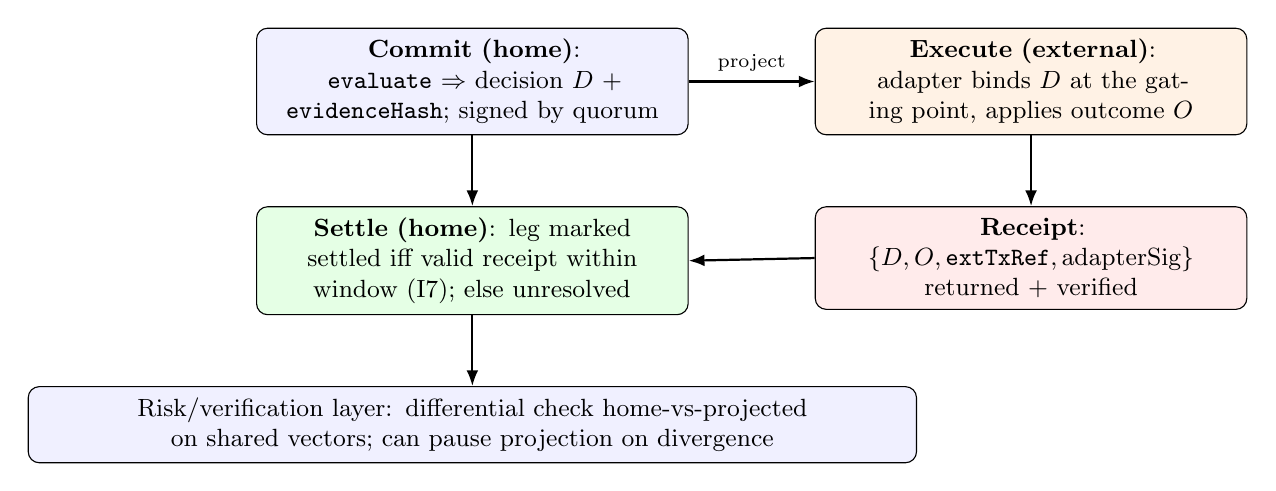
\begin{tikzpicture}[
  node distance=6mm,
  fbox/.style={draw, rounded corners, fill=blue!6, align=center, text width=52mm, inner sep=4pt, font=\small},
  hbox/.style={draw, rounded corners, fill=green!10, align=center, text width=52mm, inner sep=4pt, font=\small},
  xbox/.style={draw, rounded corners, fill=orange!10, align=center, text width=52mm, inner sep=4pt, font=\small},
  rbox/.style={draw, rounded corners, fill=red!8, align=center, text width=52mm, inner sep=4pt, font=\small},
  arr/.style={-{Latex[length=2mm]}, thick},
]
\node[fbox] (s1) {\textbf{Commit (home)}: \texttt{evaluate} $\Rightarrow$ decision $D$ + \texttt{evidenceHash}; signed by quorum};
\node[xbox, right=16mm of s1] (s2) {\textbf{Execute (external)}: adapter binds $D$ at the gating point, applies outcome $O$};
\node[rbox, below=9mm of s2] (s3) {\textbf{Receipt}: $\{D, O, \texttt{extTxRef}, \text{adapterSig}\}$ returned + verified};
\node[hbox, below=9mm of s1] (s4) {\textbf{Settle (home)}: leg marked settled iff valid receipt within window (I7); else unresolved};
\node[fbox, below=9mm of s4, text width=110mm] (s5) {Risk/verification layer: differential check home-vs-projected on shared vectors; can pause projection on divergence};

\draw[arr] (s1.east) -- node[above,font=\scriptsize]{project} (s2.west);
\draw[arr] (s2) -- (s3);
\draw[arr] (s3.west) -- (s4.east);
\draw[arr] (s4) -- (s5);
\draw[arr] (s1.south) -- (s4.north);
\end{tikzpicture}
\caption{Commit/execute with an enforcement receipt. The home ledger gives an
atomic guarantee; the external leg is settled only against a verified receipt
(\Iref{7}). The risk layer independently checks that projected decisions match
home decisions and can halt projection --- format-identity (conformance) is
upgraded to enforcement-identity (receipt).}
\label{fig:deploy}
\end{figure}

\begin{lstlisting}[caption={The enforcement receipt closes the loop: a projected
decision is settled only when its application is proven, not when it is
sent.},captionpos=b]
struct EnforcementReceipt {
    bytes32 decisionHash;   // = H(D)
    bytes32 evidenceHash;   // must equal the home commitment (I6, I7)
    uint8   outcome;        // applied PERMIT / DENY at the external gating point
    bytes32 extTxRef;       // external ledger transaction reference
    bytes   adapterSig;     // adapter / external attester signature
}
\end{lstlisting}

Two honest points carry over and are now bounded rather than waved away.
\emph{Atomicity}: cross-ledger DvP is only as strong as the connector's
coordination (\Aref{5}); on public ledgers this interacts with probabilistic
finality, so the home guarantee is strictly stronger and \Iref{7} marks an
unreceipted leg \emph{unresolved}, not settled. \emph{Adapter weight}: external
adapters for UTXO, partitioned (ERC-1400) and Corda notary models are not thin,
and the receipt requirement adds work --- but it buys a property conformance alone
cannot give.

\subsection{Quantity correctness across ledgers}
A freeze projects cleanly because it is boolean: a freeze denies on both venues
from the one instance (\Iref{5}). A \emph{holder cap} does not, because it is a
quantity over \emph{aggregate} holdings, and naive projection lets a party sit
under the cap on each ledger while breaching it in total. Invariant~\Iref{8}
fixes this: one ledger (the home contract) holds the canonical counter, and a
cross-ledger acquisition follows \texttt{reserve}~$\rightarrow$~confirm against it
--- reserve headroom before the external move, commit on receipt, release on
timeout. Concurrency cannot breach the aggregate bound. Where a cap is genuinely
per-venue, it is declared single-ledger explicitly. Either way the design no
longer implies a quantity guarantee it cannot keep.

% =====================================================================
\section{Standards, conformance and governance on Swift's terms}
\label{sec:conformance}

\subsection{Conformance becomes certification with golden vectors}
The portable design's proof of asset-agnosticism --- identical decisions for
identical requests across adapters --- becomes a Swift-native, executable
certification. We publish on MyStandards, alongside the request/decision schema
and reason-code dictionary, a corpus of \textbf{golden test vectors}: tuples
$(\texttt{request} \rightarrow \texttt{decision}, \texttt{reasonCode},
\texttt{evidenceHash})$ that every adapter must reproduce. The Readiness Portal
runs them exactly as banks test ISO~20022 readiness today~\cite{swiftmystd}. The
suite asserts:
\begin{itemize}[leftmargin=1.4em,itemsep=2pt]
  \item \textbf{Decision determinism} --- same request, same decision and
  \texttt{evidenceHash}, on home and every adapter.
  \item \textbf{Differential home-vs-projected} --- the corpus run against the
  external adapter must match the home result, which is what the risk layer of
  Section~\ref{sec:deploy} enforces at runtime (\Iref{7}).
  \item \textbf{Negative tests} --- fail-closed on malformed/missing attestation
  (\Iref{1}), replay rejection (\Iref{4}), epoch-floor rejection (\Iref{3}),
  freeze dominance (\Iref{5}), binding-revocation rejection and its stickiness
  against a re-screen (\Iref{9}), and per-asset policy divergence (a bond corpus
  and a deposit corpus produce different, correct decisions;
  Section~\ref{sec:policy}).
\end{itemize}
Certification is thus passing a versioned vector set, not running a bespoke
harness --- an artefact in the platform institutions already use for onboarding.

\subsection{ISO 20022 reason codes and candidate extensions}
Permitted and denied outcomes reuse the external status-reason code sets,
patterned on \texttt{pacs.002}; holding changes on \texttt{camt.054}; identity on
IVMS101. Where the digital-asset domain needs vocabulary ISO~20022 lacks --- a
token-level freeze status, the wallet-to-BIC binding, and the epoch/evidence
metadata of this design --- these are proposed as candidate extensions through
SMPG/PMPG, the same route every change to the standard travels~\cite{swiftsmpg}.

\subsection{Lifecycle, oversight and the operator boundary}
Rule and registry changes (policy modules, signer keys, epoch floors) follow
propose~$\rightarrow$~review~$\rightarrow$~threshold-approve~$\rightarrow$~time-locked
activation~$\rightarrow$~active~$\rightarrow$~deprecate, every transition emitting
an event. Two points sharpen the governance:
\begin{itemize}[leftmargin=1.4em,itemsep=2pt]
  \item \textbf{Operator $\ne$ custodian.} Swift operates the ledger and the
  signer but banks hold keys and assets~\cite{swiftmvp}. The function can
  \emph{deny}, \emph{emit} and (with authorisation) \emph{freeze}, but never moves
  or holds value --- keeping the emergency-freeze power accountable and bounded.
  \item \textbf{Security baseline.} Participants already operate under Swift's
  Customer Security Programme; the signer-quorum key custody, the
  epoch-advance authority, and audit retention are stated as extensions of that
  baseline rather than a new regime.
\end{itemize}

% =====================================================================
\section{Progressive trust-minimisation roadmap}
\label{sec:roadmap}

We do not claim the end-state on day one. We state the trust we concentrate now
and the path that reduces it --- the discipline an interoperability protocol team
applies to its own decentralisation.
\begin{description}[leftmargin=2.6em,itemsep=2pt]
  \item[\textbf{S0} (today; demo).] Single Swift HSM signer; static config; epoch
  floors, evidence commitments and sticky binding revocation (\Iref{9}) live.
  Fully buildable in the hackathon sandbox.
  \item[\textbf{S1}.] $M$-of-$N$ threshold ECDSA quorum within Swift; on-chain
  signer registry with rotation; epoch-bound freshness and binding lifecycle in
  production; validator-set governance documented (Section~\ref{sec:sequencing}).
  \item[\textbf{S2}.] Independently audited quorum; the cross-ledger risk layer
  live; separately governed break-glass set; published certification vectors;
  transaction-graph confidentiality hardened via Besu privacy groups
  (Section~\ref{sec:graph-confidentiality}).
  \item[\textbf{S3}.] Diversified attester set (potentially including non-Swift
  participants) for the risk layer and a more decentralised validator set; the
  \texttt{InvestorEligibility} module standardised through SMPG so the investor-KYC
  gap is closed by market practice rather than left open; commitment/ZK selective
  disclosure for amounts where confidentiality requires it.
\end{description}
The single biggest concentrated trust --- the PIP oracles (\Aref{4}) and the CA
(\Aref{2}) --- is named, not engineered away; it is the asset governance must
audit, and S2--S3 reduce its blast radius rather than pretend it is absent.

% =====================================================================
\section{Worked example: the trial scenario, made native}
\label{sec:example}

Take the scenario Swift trialled in January~2026: DvP settlement of a tokenised
bond using SG-FORGE's platform and its EURCV stablecoin, across paying-agent,
custodian and registrar roles~\cite{fstrial,swiftledgerpr}.

\begin{enumerate}[leftmargin=1.5em,itemsep=2pt]
  \item The buyer institution has its KYC in the Registry and has signed a
  \texttt{WalletBinding}; a Swift relay has cached a \texttt{PARTY\_STANDING}
  attestation stamped with the current \texttt{registryEpoch} and an
  \texttt{evidenceHash}.
  \item The operation is requested. The engine loads the \emph{bond} policy
  (allowlist, freeze, holder cap, lock-up, sanctions, jurisdiction --- a deposit
  would load fewer). The Besu fast path confirms standing freshness against the
  epoch floors, an unfrozen holding, and an intact cap.
  \item Transaction Screening evaluates sanctions/jurisdiction; the threshold
  signer returns a ``clear'' attestation at the current \texttt{listEpoch},
  committing an \texttt{evidenceHash} over the list epoch and ruleset version.
  \texttt{evaluate} verifies it recovers to an active signer-registry key.
  \item Under deny-overrides all modules permit; the PEP commits the asset leg in
  the same operator-coordinated step as the EURCV funding check, and emits
  \texttt{ControlDecisionLogged} with the \texttt{evidenceHash} (\Iref{6}).
  \item A \texttt{pacs.002}-patterned status notification carrying IVMS101
  originator/beneficiary data is emitted over Swift to both back offices for
  reconciliation.
\end{enumerate}

\noindent
\textbf{Freeze variant.} A regulator orders a freeze on the seller. The operator
records \texttt{FreezeOrdered}; the function emits \texttt{FreezeApplied}. On the
seller's next transfer the live on-chain freeze flag denies (\Iref{5})
\emph{regardless} of any outstanding ``clear''; if the seller also holds the bond
as an ERC-3643 token externally, the projected decision denies there too and the
home leg requires a receipt confirming it (\Iref{7}).

\noindent
\textbf{Sanctions-update variant.} The seller is added to a sanctions list at
\texttt{listEpoch}~$e+1$. Sanctions List Monitor's alert drives one
\texttt{advanceListEpoch(e+1)}. The seller's cached ``clear@$e$'' is now below the
floor; the next operation forces a re-screen, which denies --- no per-party revoke
message and no wait for \texttt{validUntil} (\Iref{3}).

\noindent
\textbf{Binding-revocation variant.} The institution controlling the seller's
wallet is offboarded --- its 3SKey credential is revoked (chaining to \Aref{2}).
The operator calls \texttt{revokeBinding}. The seller's next operation denies
\texttt{BND13} (\Iref{9}). The discriminating point: even after the routine
re-screen re-stamps every clean party at the current \texttt{listEpoch}, the
seller stays denied --- the kill is on the \emph{binding}, not the screening, so a
re-screen cannot lift it. Only the institution re-signing a \texttt{WalletBinding}
at a higher \texttt{bindingEpoch} (a \texttt{rebind}) restores standing. This is
the sanctions-update variant's mirror image: there a re-screen \emph{heals} the
deny; here it must \emph{not}.

% =====================================================================
\section{Security and operational deltas specific to Swift}
\label{sec:security}

The companion design's analysis of replay, adversarial ordering, execution cost
and availability is now subsumed by the invariants of Section~\ref{sec:trust}.
Five Swift-specific deltas remain:
\begin{itemize}[leftmargin=1.4em,itemsep=2pt]
  \item \textbf{Operator concentration and sequencing.} Routing signing through a
  Swift quorum concentrates trust in Swift. This matches Swift's
  neutral-orchestrator role and CA function, and \Aref{3} bounds single-node
  power. The distinct worry --- that the operator could also abuse its
  \emph{sequencing} position --- is bounded structurally by QBFT: ordering is
  committed by a validator super-majority, not the operator, so it is accountable
  and attributable (Section~\ref{sec:sequencing}). Both are deliberate
  centralisations addressed over time by S2--S3 (Section~\ref{sec:roadmap}).
  \item \textbf{Permissioned-ledger economics.} On Besu gas is immaterial and
  cold-path verification is negligible relative to the value in scope, so the
  ``uneconomical for small transfers'' concern of the portable design evaporates.
  The binding-liveness check (\Iref{9}) adds two storage reads per leg --- real,
  measured, and immaterial here.
  \item \textbf{Atomicity asymmetry.} Home DvP is atomic (\Iref{1}); cross-ledger
  DvP is receipt-verified but only as atomic as the connector (\Aref{5}). Risk
  statements must distinguish the two --- \Iref{7} encodes the difference.
  \item \textbf{Transaction-graph visibility.} The permissioned ledger exposes the
  pseudonymous graph to validators (not the public); the control function adds no
  leakage beyond what shared settlement requires. Posture and mitigations are
  stated explicitly in Section~\ref{sec:graph-confidentiality}.
  \item \textbf{Liveness under signer outage.} Cached standing keeps working
  during a quorum outage; only a first-ever screening of a never-seen counterparty
  blocks (fail-closed, \Iref{1}). Proactive issuance for active participants keeps
  this residual small --- the same irreducible case the portable design identifies.
\end{itemize}

% =====================================================================
\section{Limitations and open questions}
\label{sec:limits}

\begin{itemize}[leftmargin=1.4em,itemsep=2pt]
  \item \textbf{Investor-level KYC is out of Registry scope.} The wallet-to-BIC
  binding covers institutional eligibility; investor accreditation is the holding
  institution's responsibility, modelled as the \texttt{InvestorEligibility}
  module and only closed at S3.
  \item \textbf{The threshold signer is a proposal, not a product.} The
  cryptography is mature and the CA exists, but a Swift-operated threshold module
  is not a published service; standing it up is an operational project with its
  own assurance requirements.
  \item \textbf{The PIP oracles are trusted (\Aref{4}).} Correctness of sanctions
  and registry results is assumed, not proven. Evidence commitments (\Iref{6})
  make outcomes \emph{auditable} after the fact but do not remove the trust; only
  diversified attestation (S3) reduces it.
  \item \textbf{Epoch freshness bounds, does not eliminate, latency.} An
  \texttt{advanceListEpoch} still has to land in a block; the window is bounded by
  block time, not zero.
  \item \textbf{Cross-ledger atomicity is bounded by the connector (\Aref{5}).}
  Receipts upgrade format-identity to enforcement-identity but inherit the
  connector's settlement guarantees, which on public ledgers interact with
  probabilistic finality.
  \item \textbf{Canonical counters add a home dependency.} Quantity correctness
  (\Iref{8}) routes cross-ledger fungible caps through the home counter, trading
  some external autonomy for aggregate safety.
  \item \textbf{Registry coverage is not universal.} Not every counterparty
  (especially non-bank or retail-facing) is present; the eligibility PIP degrades
  to ``unknown $=$ deny,'' which is safe (\Iref{1}) but can over-block.
  \item \textbf{Transaction-graph confidentiality is bounded, not closed.} The
  permissioned ledger keeps the pseudonymous graph from the public but not from
  validators; \texttt{walletRef} rotation and Besu privacy groups reduce, and
  commitment/ZK disclosure (S2--S3) further reduce, but do not yet eliminate,
  intra-set linkability (Section~\ref{sec:graph-confidentiality}).
  \item \textbf{Binding revocation relies on timely governance signals.} Sticky
  revocation (\Iref{9}) collapses removal latency to one write, but it still
  depends on the offboarding / credential-revocation event reaching the operator;
  the on-chain mechanism is immediate, the upstream notification is not free.
\end{itemize}

% =====================================================================
\section{Conclusion}
\label{sec:concl}

The portable control function answers ``how do we make one compliance control
work across any ledger?'' This specialisation answers the question Swift's stack
poses --- ``how do we make that control native to Swift, using what Swift has
already built?'' --- and answers it the way a protocol team would: almost every
off-chain box has a real Swift home, the one new artefact is a signed
wallet-to-BIC binding --- now with a sticky revocation lifecycle (\Iref{9}) ---
and every guarantee is stated as an invariant conditional on a named assumption.
The upgrades that matter are structural, not cosmetic: epoch-bound freshness turns
the worst residual risk into a one-write safety property; a per-asset policy
registry makes asset-agnosticism constructed rather than claimed; evidence
commitments make decisions auditable; a governed signer registry handles key
lifecycle; and enforcement receipts upgrade cross-ledger projection from formatted
to verified. The three gaps a protocol review flags are closed in kind, not waved
away: the binding now revokes stickily, operator sequencing is shown accountable
under QBFT rather than assumed, and transaction-graph confidentiality is given an
explicit posture. We remain explicit about the three places --- investor KYC, a
productised signer, trusted PIP oracles --- where the design depends on work Swift
has not yet shipped, and we give the roadmap that reduces that trust over time
rather than asserting it away.

% =====================================================================
\begin{thebibliography}{99}
\small
\bibitem{swiftledgerpr} Swift, \emph{Swift to add a blockchain-based shared ledger to its infrastructure stack} (29 Sep.\ 2025). \url{https://www.swift.com/news-events/press-releases/swift-add-blockchain-based-ledger-its-infrastructure-stack-groundbreaking-move-accelerate-and-scale-benefits-digital-finance}
\bibitem{swiftmvp} Swift, \emph{Swift's blockchain-based shared ledger progresses to MVP implementation} (30 Mar.\ 2026) --- EVM-compatible, Hyperledger Besu; Swift operates, banks hold keys. \url{https://www.swift.com/news-events/news/swifts-blockchain-based-shared-ledger-progresses-mvp-implementation}
\bibitem{fstrial} FStech, \emph{Swift plans blockchain-based shared ledger after `landmark' digital asset trial} (15 Jan.\ 2026) --- DvP of tokenised bonds with BNP Paribas, Intesa Sanpaolo, SG-FORGE. \url{https://www.fstech.co.uk/fst/Swift_Plans_Blockchain_Based_Shared_Ledger_After_Landmark_Digital_Asset_Trial.php}
\bibitem{swiftkyc} Swift, \emph{KYC Registry} (BIC-keyed institutional due diligence; owner-controlled access and audit trail). \url{https://www.swift.com/products/kyc-registry}
\bibitem{swiftkycdata} Swift, \emph{The KYC Registry continues to foster trust across our community} (API real-time monitoring; ISSA DDQ securities module). \url{https://www.swift.com/news-events/news/kyc-registry-continues-foster-trust-across-our-community}
\bibitem{swifttxnscreen} Swift, \emph{Transaction Screening} (real-time sanctions screening; Smart Screening uses ISO 20022). \url{https://www.swift.com/products/transaction-screening}
\bibitem{swiftslm} Swift, \emph{Sanctions List Monitor} (instant standardised alerts on sanctions-list changes). \url{https://www.swift.com/products/sanctions-list-monitor}
\bibitem{swift3skey} Swift, \emph{3SKey} (multi-bank personal digital identity; PKI; key-share signing). \url{https://www.swift.com/products/3skey}
\bibitem{swiftpki} Swift, \emph{Swift Certificate Centre / Swift PKI} (Swift Root CA; certification services). \url{https://www.swift.com/interfaces-and-integration/swift-certificate-centre}
\bibitem{swift3skeyfs} Swift, \emph{3SKey for Banks --- factsheet} (PKI; device-bound key-share model; FIPS 140-2 tokens). \url{https://www2.swift.com/3skey/documents/SWIFT_3SKey_for_banks_factsheet.pdf}
\bibitem{swiftmystd} Swift, \emph{MyStandards} (publish/test ISO 20022 usage guidelines; Readiness Portal; 150+ publishing organisations). \url{https://www.swift.com/products/mystandards}
\bibitem{swiftsmpg} Swift, \emph{ISO 20022 standards and market practice} (SMPG/PMPG/CBPR+ governance). \url{https://www.swift.com/standards/iso-20022/iso-20022-standards}
\bibitem{swiftchainlink23} Swift, \emph{Swift unlocks potential of tokenisation with successful blockchain experiments} (Chainlink as enterprise abstraction layer; CCIP for interoperability). \url{https://www.swift.com/news-events/press-releases/swift-unlocks-potential-tokenisation-successful-blockchain-experiments}
\bibitem{swiftcbdc} Swift, \emph{Swift sets industry up for seamless introduction of CBDCs} (interlinking connector; atomic DvP across networks). \url{https://www.swift.com/news-events/press-releases/swift-sets-industry-seamless-introduction-cbdcs-cross-border-transactions-interlinking-solution-finds-more-use-cases}
\end{thebibliography}

\end{document}
